%\documentclass[margin=0pt]{standalone}
%\usepackage{tikz}
\usetikzlibrary{backgrounds}

\begin{document}

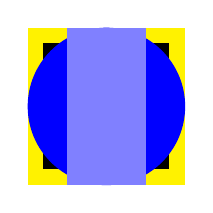
\begin{tikzpicture}
    % On main layer:
    \fill[blue] (0,0) circle (1cm);
    \begin{scope}[on background layer={color=yellow}]
        \fill (-1,-1) rectangle (1,1);
    \end{scope}
    \begin{scope}[on background layer]
        \fill[black] (-.8,-.8) rectangle (.8,.8);
    \end{scope}
    % On main layer again:
    \fill[blue!50] (-.5,-1) rectangle (.5,1);
\end{tikzpicture}

\end{document}
